
%(BEGIN_QUESTION)
% Copyright 2012, Tony R. Kuphaldt, released under the Creative Commons Attribution License (v 1.0)
% This means you may do almost anything with this work of mine, so long as you give me proper credit

Although not standard practice, it is possible to build a proportional-only control system using nothing but a transmitter, an I/P converter, and a control valve.  Here is an example on a gas pressure control system, where the control valve vents excess gas from the vessel in order to maintain gas pressure inside the vessel at a relatively constant value:

$$\includegraphics[width=15.5cm]{i01108x01.eps}$$

Explain how you could vary the {\it gain} of this ``control system'' without adding or replacing any components, but merely making adjustments to the components already installed:

\vskip 50pt

Explain how you could vary the {\it setpoint} of this ``control system'' without adding or replacing any components, but merely making adjustments to the components already installed:

\vskip 50pt

\underbar{file i01108}
%(END_QUESTION)





%(BEGIN_ANSWER)

To change the gain of the system, you would have to change the gain of any one component.  Examples include:

\begin{itemize}
\item{} Adjust span of transmitter
\item{} Adjust span of I/P
\end{itemize}

\vskip 10pt

To change the setpoint, you would have to change the bias of any one component.  Examples include:

\begin{itemize}
\item{} Adjust zero of transmitter
\item{} Adjust zero of I/P
\item{} Adjust spring tension (lower bench set value) of control valve
\end{itemize}

%(END_ANSWER)





%(BEGIN_NOTES)

{\bf This question is intended for exams only and not worksheets!}.

%(END_NOTES)


